%% main.tex — data_redactor performance experience report.
%% Target: arXiv (acmart, [acmsmall] for a single-column journal-style preprint),
%% then port to Wiley WileyNJD-v2 for Software: Practice & Experience.
%% Build: `make` (needs texlive + latexmk; see paper/Makefile). Not yet compiled
%% locally — toolchain not installed at scaffold time.
%%
%% Structure follows paper/README.md §7. Section bodies are stubs marked TODO;
%% the figures, the generated table, and the bibliography are already wired so the
%% scaffold compiles to a real skeleton once a toolchain exists.
\documentclass[acmsmall,nonacm,screen]{acmart}

%% nonacm: this is a preprint, not an ACM-copyright submission. Drop for a real
%% ACM venue. acmsmall: single-column journal layout (closest to S:P&E shape, and
%% fine for arXiv). Swap the whole \documentclass for WileyNJD-v2 at S:P&E time.

\usepackage{booktabs}   % the generated table uses \toprule/\midrule/\bottomrule
\usepackage{graphicx}
\usepackage{siunitx}     % aligned numeric columns later if wanted

\begin{document}

\title{The Fastest Engine Is Not the Shippable Engine: Replacing a
Regex Engine for Data Redaction Under Production Constraints}

%% Sole author + AI disclosure (paper/README.md §4). Fill affiliation/email.
\author{Daniele Frisanco}
\affiliation{%
  \institution{TODO: affiliation}
  \country{TODO}}
\email{daniele.frisanco@gmail.com}

\renewcommand{\shortauthors}{Frisanco}

\begin{abstract}
%% Opener locked in paper/README.md §1 (draft B). Keep the four constraints and
%% the "performance objective subject to constraints" shape. TODO: tighten to
%% ~150 words and add the headline result once the clean re-run lands.
We report on replacing the regex engine behind a data-redaction library to
improve performance under four production constraints---zero runtime
dependencies, byte-for-byte-identical output to the incumbent, robustness across
all match densities, and thread-safety in a managed runtime---and find, across a
sequence of prototypes, that the speed-optimal engine is ruled out by those
constraints, and that the pre-filter pipeline usually assumed best for
multi-pattern matching does not hold across densities; the best shippable design
is a per-pattern lazy DFA with two domain-specific merges.
\end{abstract}

%% TODO: pick CCS concepts + keywords near submission.
\keywords{regular expressions, multi-pattern matching, data redaction,
lazy DFA, performance engineering, Ruby C extensions}

\maketitle

\section{Introduction}
\label{sec:intro}
%% The hook (paper/README.md §1): the incumbent is a pure-Ruby gsub loop; the C
%% extension meant to be faster was ~5x SLOWER (0.2x). Frame as a CATEGORY ERROR,
%% not a language result: the variable was the regex engine, not C-vs-Ruby (glibc
%% regexec's O(N) per-call state-log allocation vs Onigmo's BM + O(1) stack).
%% Then: objective (performance) subject to constraints; contributions list.
\textbf{TODO.} Hook + objective/constraints + contributions.

\section{Background}
\label{sec:background}
%% Data redaction; the 88-pattern set; the pure-Ruby baseline; why a C extension
%% was expected to win (and why that expectation was a category error).
\textbf{TODO.}

\section{The Constraint Box}
\label{sec:constraints}
%% Three binary GATES (zero-dep, exact-output, thread-safe) + the all-density
%% objective. Why each gate disqualifies an attractive option: PCRE2 JIT fails
%% zero-dep; the merged NFA fails exact-output (31\%); prototype globals failed
%% thread-safety until the per-thread refactor.
\textbf{TODO.}

\section{Method: The Prototype Search}
\label{sec:method}
%% The ladder of prototypes; how each was measured; the exact-output oracle
%% (byte-for-byte vs Ruby gsub over ~6000 inputs); the four payloads + the
%% continuous density sweep. Environment from paper/data/environment.md.
\textbf{TODO.}

\section{Findings}
\label{sec:findings}

\subsection{The incumbent's cost is allocation, not a missing pre-filter}
\label{sec:finding-alloc}
%% glibc regexec O(N) per-call state-log allocation is the dominant factor, not
%% the missing Boyer-Moore. ~88 MB allocated per redact call at 88 patterns x 1MB.
%% Figure~\ref{fig:overview} shows the reproduced glibc baseline ~8-10x slower
%% than pure-Ruby across the density range.
\textbf{TODO.}

\begin{figure}[t]
  \centering
  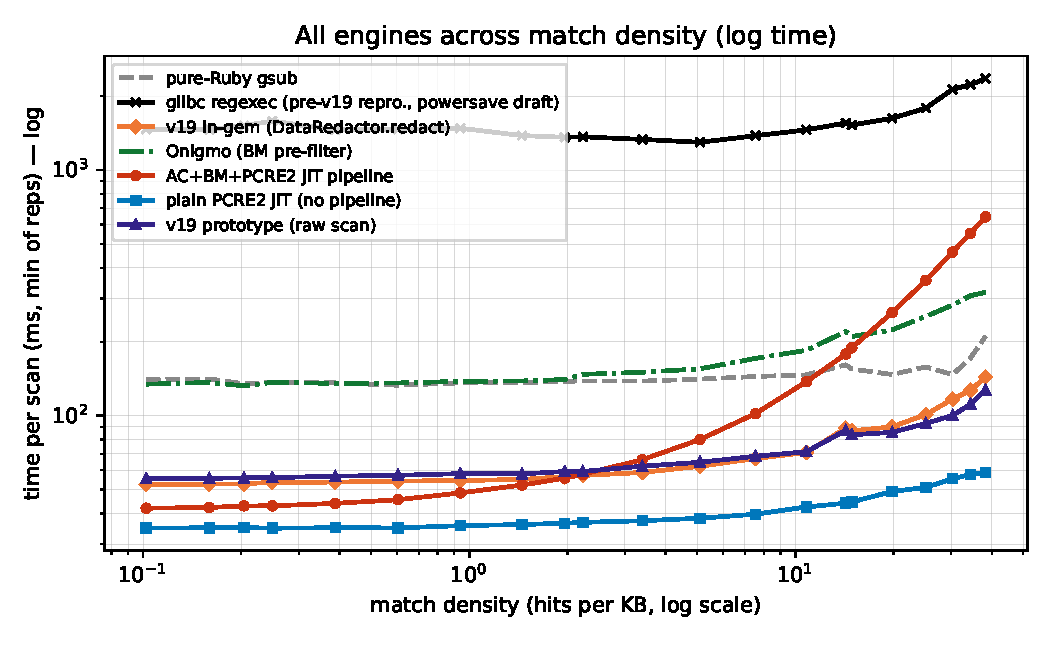
\includegraphics[width=\linewidth]{figures/density_overview.pdf}
  \caption{Time per scan vs.\ match density (log--log), all engines. The
  reproduced pre-v19 glibc \texttt{regexec} engine is \(\sim\)8--10\(\times\)
  slower than the pure-Ruby \texttt{gsub} loop it was meant to beat. DRAFT data:
  single session, shared machine under the \texttt{powersave} governor; shape is
  trustworthy, absolute magnitudes pending a clean re-run.}
  \label{fig:overview}
\end{figure}

\subsection{The pre-filter pipeline penalty grows with match density}
\label{sec:finding-crossover}
%% The money figure. Mechanism stated generally, magnitude locally (README §5):
%% a literal/AC pre-filter pays off only by REJECTING positions; as more
%% positions carry a hit, fewer are rejected, so the per-position cost is paid
%% without the skip benefit. The AC+BM+JIT pipeline is strictly dominated by the
%% same JIT without the pipeline at every sampled density (1.15x sparse -> 10.6x
%% dense), and overtakes pure-Ruby at ~12 hits/KB. Onigmo (also BM-pre-filtered)
%% climbs too -- independent corroboration. Scope every claim to our config.
\textbf{TODO.}

\begin{figure}[t]
  \centering
  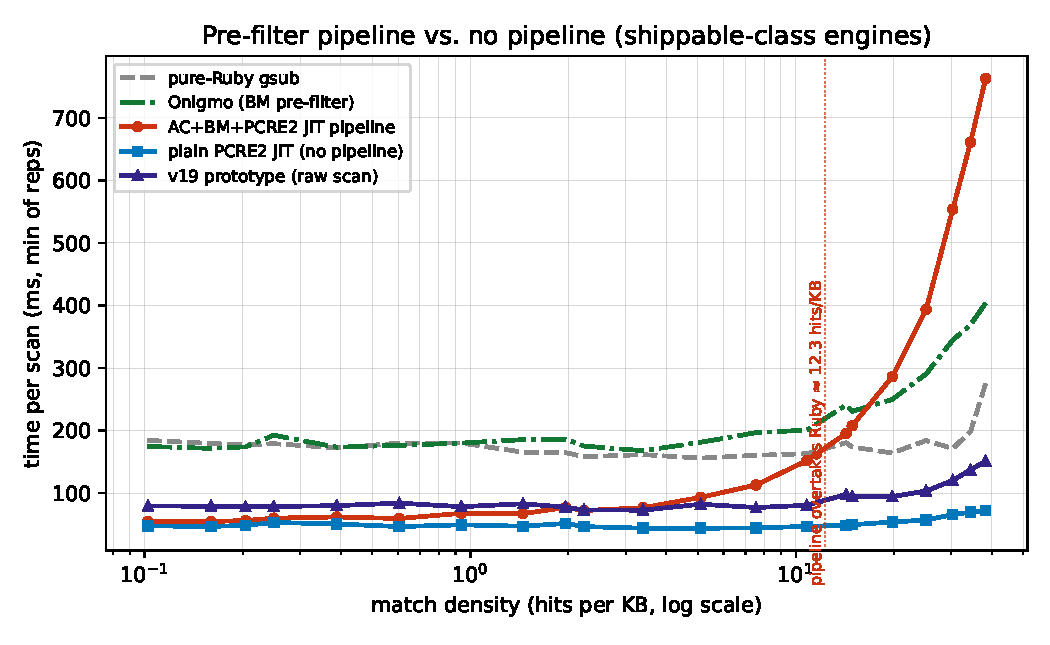
\includegraphics[width=\linewidth]{figures/density_crossover.pdf}
  \caption{Time per scan vs.\ match density (shippable-class engines, linear
  \(y\)). The AC+BM+PCRE2-JIT pipeline tracks the no-pipeline engines when hits
  are rare, then its cost rises with density and overtakes the pure-Ruby baseline
  at \(\approx 12\) hits/KB. Plain PCRE2 JIT and the v19 lazy-DFA engine stay flat.
  DRAFT data (see Fig.~\ref{fig:overview}).}
  \label{fig:crossover}
\end{figure}

\begin{table}[t]
  \centering
  \caption{Time per scan (ms, min of reps) at selected densities. Generated by
  \texttt{paper/plot\_density\_sweep.py}; DRAFT data.}
  \label{tab:density}
  % generated by paper/plot_density_sweep.py — do not hand-edit
\begin{tabular}{rrrrrrrr}
\toprule
hits/KB & pure-Ruby gsub & glibc regexec & v19 in-gem & Onigmo & AC+BM+PCRE2 JIT pipeline & plain PCRE2 JIT & v19 prototype \\
\midrule
38.28 & 274.7 & 2360.5 & 176.5 & 403.8 & 763.1 & 72.0 & 151.2 \\
14.27 & 180.6 & 1554.9 & 97.1 & 240.8 & 195.6 & 48.5 & 97.8 \\
1.96 & 164.7 & 1360.3 & 69.7 & 186.3 & 77.0 & 51.4 & 77.6 \\
0.20 & 176.9 & 1516.2 & 72.4 & 173.9 & 56.1 & 48.4 & 78.3 \\
0.10 & 184.3 & 1466.2 & 72.7 & 174.6 & 54.6 & 47.5 & 79.3 \\
\bottomrule
\end{tabular}

\end{table}

\subsection{The shippable design: per-pattern lazy DFA + two selective merges}
\label{sec:finding-v19}
%% v18 lazy DFA (Cox, used as-is); v18.1 anchor lowering (88/88 on DFA); v19's two
%% selective merges (pure-digit group, IBAN union pass) framed as SPECIALIZATION,
%% not a grouping algorithm (README §5). Zero-dep, beats Onigmo on all payloads.
\textbf{TODO.}

\subsection{Prototype-to-production hardening: GVL-free re-entrancy}
\label{sec:finding-hardening}
%% The immutable/mutable state split (incl. the lazy DFA cache going per-thread),
%% GVL release for large inputs, allocation-floor + pthread_key reclaim to bound
%% per-thread RSS. The systems contribution. (research_log.md §"Prototype ->
%% production".)
\textbf{TODO.}

\section{Evaluation}
\label{sec:eval}
%% Gates first (who is eligible), then the density curve (who is fast where it
%% counts). vs Ruby / reproduced glibc / Onigmo / PCRE2 JIT.
\textbf{TODO.}

\section{Discussion and Threats to Validity}
\label{sec:discussion}
%% Scope of claims; the powersave/single-session caveat; reproduction-not-original
%% baseline; where the mechanism generalizes and where magnitudes do not.
\textbf{TODO.}

\section{Related Work}
\label{sec:related}
%% Cox lazy/hybrid DFA (used as-is). RE2::Set / Rust RegexSet state explosion past
%% ~30 patterns (the wall we avoid by per-pattern DFAs). Hyperscan (x86-only, why
%% disqualified). BLARE (closest structural cousin: extract-literal-then-confirm).
%% Explicit NON-citation of rule-grouping/partitioning heuristics -- shared
%% vocabulary, different method (research_log.md §"Related work").
\textbf{TODO.}

\section{Conclusion}
\label{sec:conclusion}
\textbf{TODO.}

%% AI-use disclosure (paper/README.md §4).
\begin{acks}
The author used Claude (Anthropic) for drafting, literature triage, and
code/benchmark implementation; the author reviewed and is responsible for all
content.
\end{acks}

\bibliographystyle{ACM-Reference-Format}
\bibliography{refs}

\end{document}
